	\clearpage
\section{Testszenarien}\label{sec:Testszenarien}

Die Benchmarks der Mesh Protokolle sollen mit unterschiedlichen Bedingungen getestet werden wobei grundsätzlich eine reelle Anwendung nachgebaut werden soll. Zum einen gibt es unterschiedliche Beziehungen innerhalb des Mesh Netzwerks, zum anderen werden Testumgebungen unterschieden.

\subsection{Mesh Beziehungen}\label{subsec:MeshBeziehungen}

Innerhalb eines Mesh Netzwerks können 4 Beziehungen zwischen den Nodes für die Benchmarks unterschieden werden. Üblicherweise kommen mehrere oder sogar alle 4 Beziehungen innerhalb eines Netzwerkes gleichzeitig zum Einsatz. Abbildung \ref{fig:MeshTestBeziehungen} zeigt die Beziehungen.

\begin{itemize}
 	\item \textcolor{red}{Rot stellt eine einfache P2P Verbindung ohne Hop dar. Beispielweise schaltet ein einzelner Schalter eine einzelne, definierte Lichtquelle}
 	\item \textcolor{orange}{Orange ist eine many-to-one Verbindung in welcher mehrere Lichtschalter die selbe Lichtquelle schalten.}
 	\item \textcolor{cyan}{In blau ist eine klassiche one-to-many Topologie dargestellt in welcher beispielsweise ein Schalter mehrere Lichtquellen bedient.}
 	 \item \textcolor{green}{Grün dargestellt ist eine indirekte P2P Verbindung mit. Das bedeutet, dass Schalter und Lichtquelle keine direkte Verbindung zueinander haben und daher Mesh-typisch via einem oder mehreren Hops kommuniziert.}
\end{itemize}


\begin{figure}[H]
	\centering
	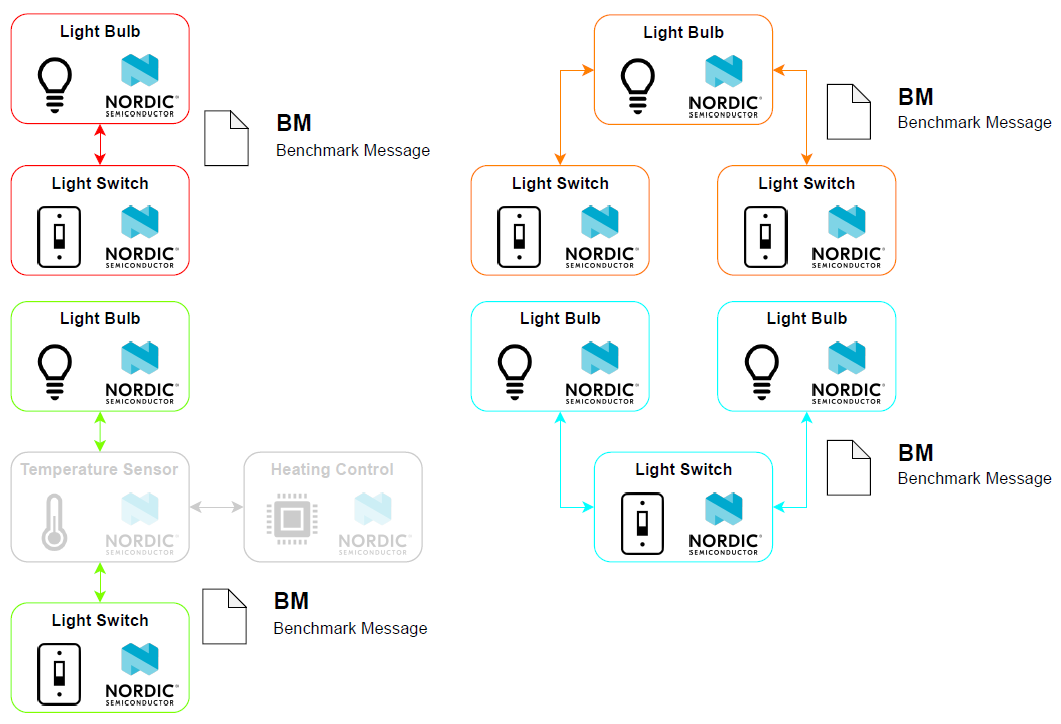
\includegraphics[width=1.0\textwidth]{Mesh_Test_Beziehungen.png}
	\caption{Beziehungen zwischen den Mesh Nodes innerhalb eines Benchmarks.}\label{fig:MeshTestBeziehungen}
\end{figure}


\subsection{Testumgebungen}\label{subsec:Testumgebungen}

Unterschiedliche Testumgebungen sollen die Benchmarks und schlussendlich den Vergleich der 3 Mesh Protokolle aussagekräftiger machen. Abbildung \ref{fig:MeshNetzwerkTestumgebungen} zeigt 5 unterschiedliche Umgebungen in denen Messungen durchgeführt werden sollen.

\begin{figure}[H]
	\centering
	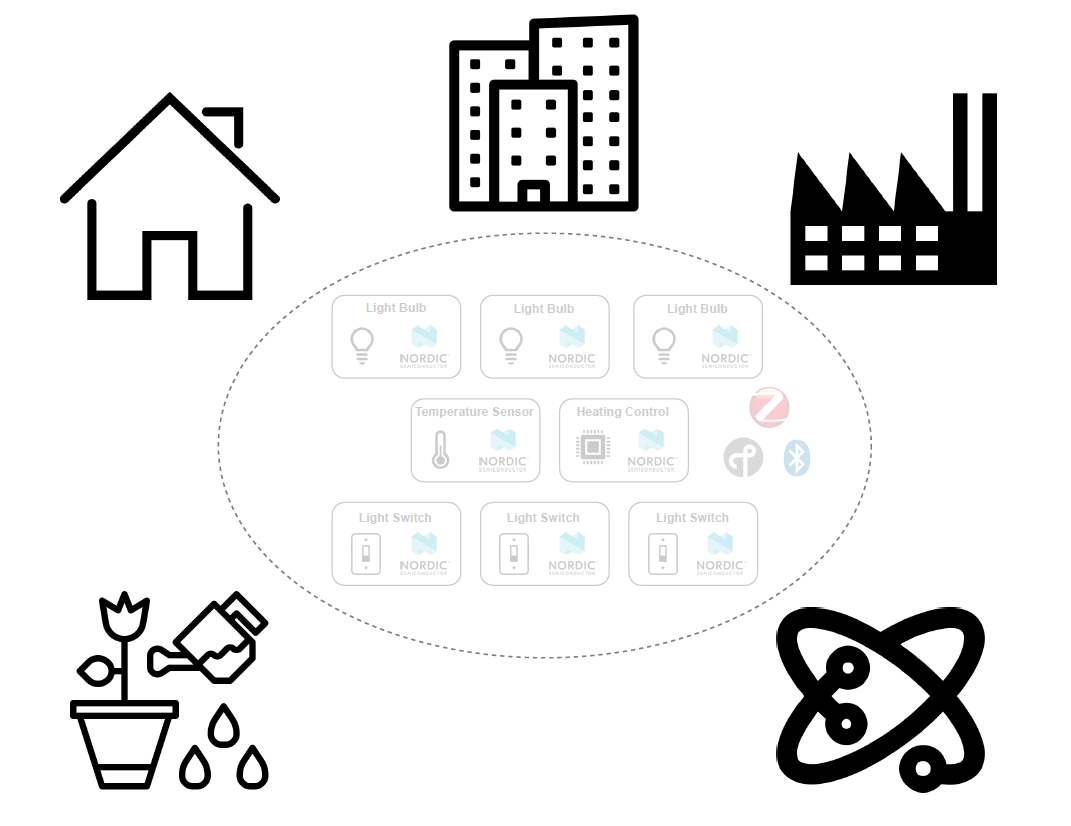
\includegraphics[width=1.0\textwidth]{Mesh_Testumgebung.png}
	\caption{Mesh Netzwerk Testumgebungen}\label{fig:MeshNetzwerkTestumgebungen}
\end{figure}

\begin{description}
\item[Haus] Die Testgeräte werden in einem Einfamilienhaus installiert und repräsentieren damit eine flächendeckende Heim-Automatisierung.
	\begin{itemize}
		\item Einfamilienhaus über mehrere Etagen.
		\item Anzahl Sensoren und Aktoren vergleichbar gross.
		\item Node-Dichte relativ gering.
		\item Keine Beeinflussung durch Nachbarsysteme zu erwarten \hfill \\
	\end{itemize}
\item[Wohnung] Ebenfalls als Heim-Automatisierung gedacht werden die Messungen in einer Wohnung durchgeführt.
	\begin{itemize}
		\item Wohnung über eine Etage in einem Mehrfamilienhaus
		\item Anzahl Sensoren und Aktoren vergleichbar gross.
		\item Node-Dichte höher als im Haus.
		\item Mögliche Störeinflüsse durch andere Systeme von Nachbarn zu 					erwarten. \hfill \\
	\end{itemize}
\item[Industrie] Um eine Industrielle Anwendung zu vergleichen erfolgt eine Messung in einem Industriebetrieb.
	\begin{itemize}
		\item Industriebetrieb mit grosser Fläche.
		\item Grosse Anzahl Sensoren zur Überwachung von Produktionsprozessen. 				Vereinzelt Aktoren zur Ansteuerung von Anlageteilen.
		\item Hohe Node-Dichte.
		\item Mögliche Störeinflüsse durch Maschinen oder Abschirmwirkung durch 			metallische Gegenstände zu erwarten. \hfill \\
	\end{itemize}
\item[Landwirtschaft (optional)] Für die Überwachung und Kontrolle von landwirtschaftlichen Flächen kann ein Test auf offenem Feld erfolgen.
	\begin{itemize}
		\item Landwirtschaftsfläche mit grosser Ausbreitung (z.B. Gemüseanbau).
		\item Grosse Anzahl Sensoren. Nur wenige bis gar keine Aktoren.
		\item Sehr geringe Node-Dichte mit weiten Distanzen.
		\item Geringe bis keine Störbeeinflussung durch die Umgebung zu erwarten. \hfill \\
	\end{itemize}
\item[Labor] Der Laboraufbau ist ein Extremtest welcher die Leistungsgrenzen der Protokollstacks ausloten soll.
	\begin{itemize}
		\item Testaufbau unter Laborbedingungen auf engstem Raum.
		\item Ausgeglichene Anzahl Sensoren und Aktoren.
		\item Sehr Hohe Node-Dichte.
		\item Geringe bis keine Störbeeinflussung durch die Umgebung zu erwarten. \hfill \\
	\end{itemize} 
\end{description}






